\section{Latar Belakang}
\label{sec:latarbelakang}

Konsumsi energi dan perkembangan ekonomi sangat berkaitan satu dengan yang lain \citep{Burke2018Impact}. Meskipun masih menjadi perdebatan di kalangan peneliti tentang hubungan kausalitas antar keduanya. Namun sejarah telah membuktikan bukti yang nyata, bahwa peningkatan aktivitas ekonomi selalu diikuti dengan meningkatnya konsumsi energi \citep{Jack2024How}. Sebelum revolusi industri, aktivitas ekonomi masih dibatasi oleh sumber energi organik seperti tenaga manusia, hewan ternak atau sinar matahari, akan tetapi setelah ditemukannya mesin uap aktivitas ekonomi berekspansi besar-besaran dengan dimungkinkannya penggunaan alat dan sistem produksi yang baru. Kelaziman tersebut juga terjadi di Indonesia dengan naiknya PDB per unit energi yang dikonsumsi tahun per tahun, hal tersebut dapat dilihat pada grafik \ref{gdp_energy_unit}.
    \begin{figure}[htbp]
		\centerline{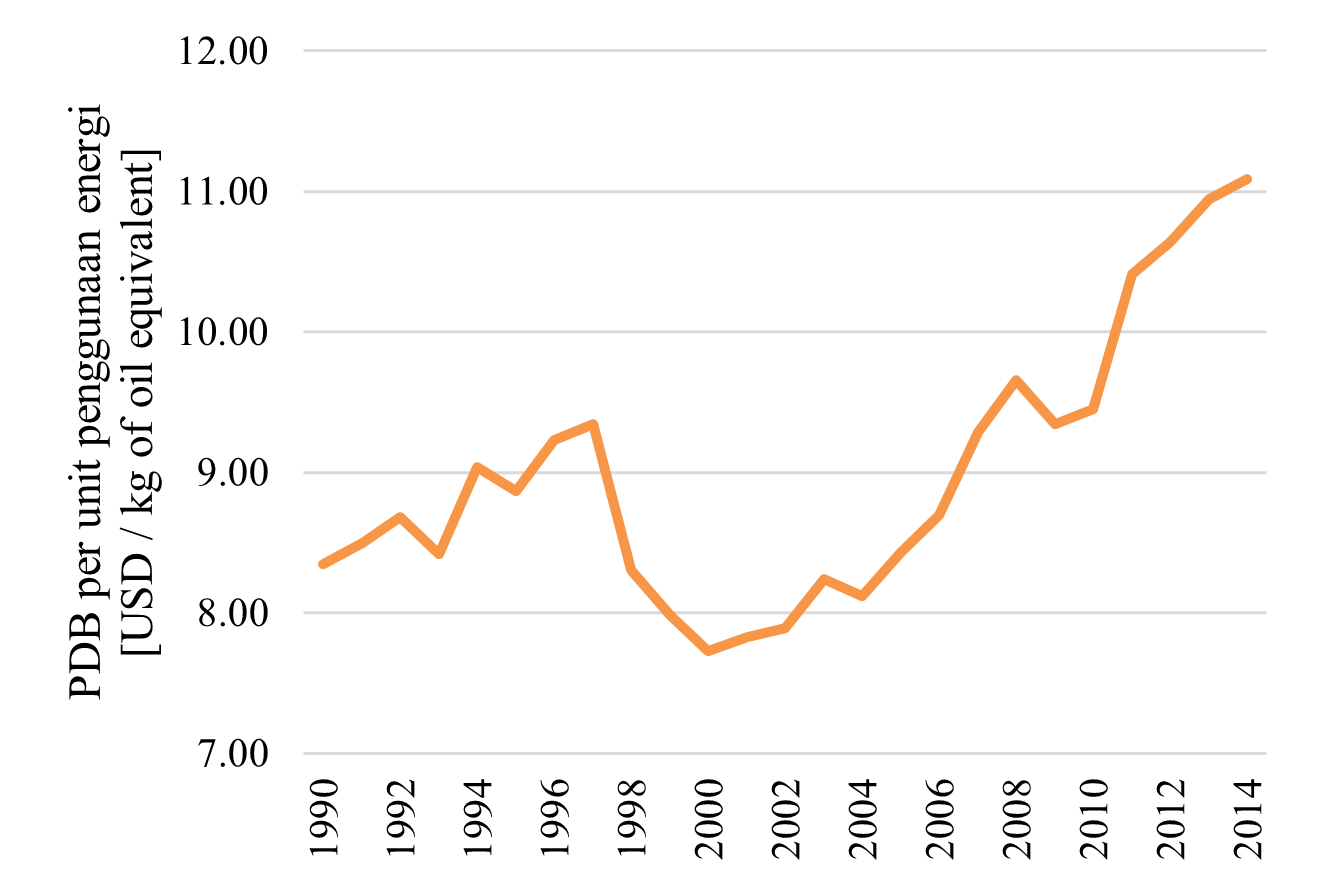
\includegraphics[width=0.75\textwidth]{grafik/gdp per unit energy consp v2.png}}
        \setlength{\belowcaptionskip}{-10pt}
		\caption{Grafik Pendapatan Domestik Bruto Indonesia per unit energi yang dikonsumsi \citep{World2024GDP}.}
		\label{gdp_energy_unit}
	\end{figure}
    
    Seperti yang ditampilkan pada grafik \ref{energy_cmix} produk olahan minyak tetap menjadi jenis energi dominan yang dikonsumsi di Indonesia, diikuti oleh listrik dan biofuel \citep{IEA2024World}. Bensin dan solar adalah jenis BBM yang paling banyak digunakan di negara ini. Namun, dominasi minyak dalam komposisi konsumsi energi menghadirkan tantangan tersendiri dalam sektor energi bagi Indonesia. Selain karena sumber energi ini tidak berkelanjutan, aksesibilitas atau kemampuan masyarakat untuk mengakses energi tersebut juga menjadi masalah.

    \begin{figure}[htbp]
		\centerline{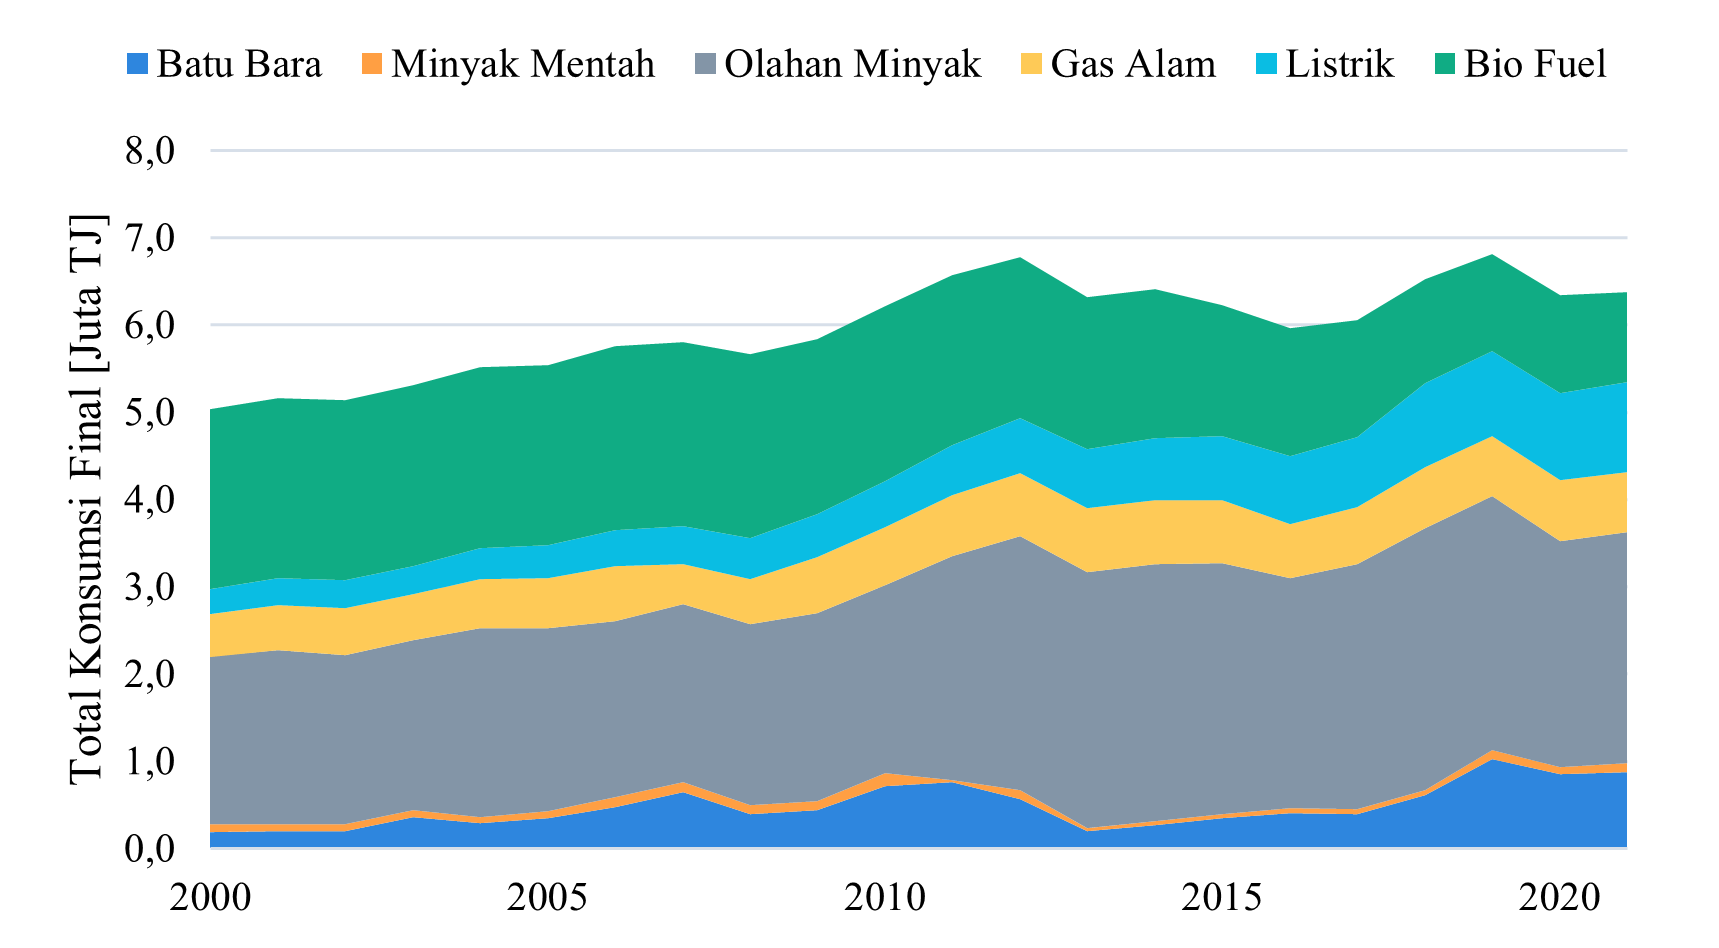
\includegraphics[width=0.75\textwidth]{grafik/komposisi_konsumsi_energi.png}}
        \setlength{\belowcaptionskip}{-10pt}
		\caption{Grafik Komposisi Konsumsi Energi Indonesia \citep{IEA2024World}.}
		\label{energy_cmix}
	\end{figure}

    Meskipun BBM merupakan jenis energi yang paling banyak digunakan, akses masyarakat terhadapnya masih tertinggal dibandingkan dengan listrik. Rasio elektrifikasi Indonesia mencapai 99,79\% pada tahun 2023 \citep{Syofiadi2024Sepanjang}, sementara aksesibilitas BBM masih jauh dari merata, mendorong pemerintah untuk berupaya mengejar ketertinggalan dan memeratakan akses BBM ke seluruh penjuru Indonesia \citep{bangun_SPBU}. Kondisi geografis Indonesia yang berupa pegunungan dan kepulauan, bersama dengan karakteristik BBM yang memerlukan distribusi dari titik produksi ke titik konsumsi, menjadi faktor utama kesenjangan akses terhadap BBM. Di sisi lain, listrik dapat diproduksi hampir di mana saja dengan adanya sumber energi dan mesin pembangkit, membuat pemerataan akses listrik lebih mudah.

    Kabupaten Maluku Barat Daya (MBD), sebuah kepulauan di sisi barat daya Kepulauan Maluku, masih bergulat dengan kesulitan akses Bahan Bakar Minyak (BBM). Kondisi kepulauan dengan jarak antar pulau yang terbentang jauh, ditambah letaknya yang lebih dekat dengan Timor Leste dibandingkan Ambon (ibukota provinsi), menjadikan MBD sebagai daerah 3TP (Tertinggal, Terluar, Terdepan, dan Perbatasan).
    
\begin{figure}[htbp]
		\centerline{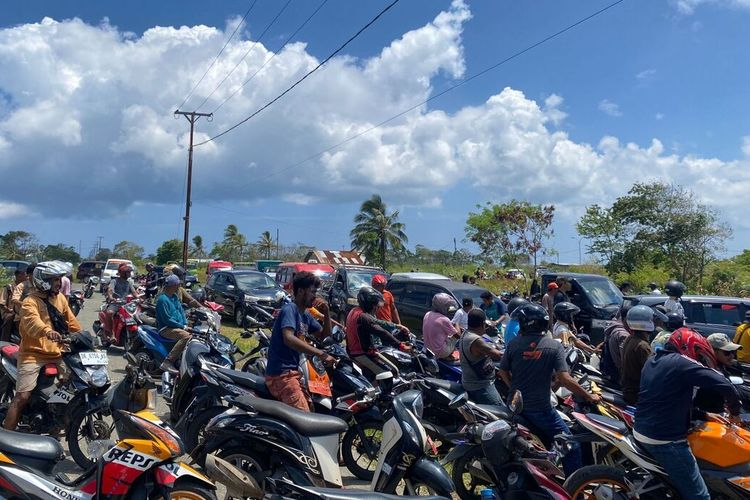
\includegraphics[width=0.7\textwidth]{gambar/antriBBM-MBD.jpg}}
        \setlength{\belowcaptionskip}{-10pt}
		\caption{Antrian Panjang Warga di  satu-satunya SPBU yang menjual BBM di Kota Tiakur \citep{Kurniati_2024}.}
		\label{antrian-bbm-mbd}
	\end{figure}
 
    Akses Bahan Bakar Minyak (BBM) di Kabupaten Maluku Barat Daya (MBD) menghadapi tantangan utama pada akses perairan. Perairan MBD merupakan perairan lepas yang berbatasan langsung dengan Laut Timor dan Samudera Hindia, sehingga tidak semua kapal dapat berlayar di wilayah tersebut. Hal ini menjadikan akses melalui perairan, yang merupakan akses utama, semakin rumit. Kelangkaan BBM di MBD kerap terjadi, terutama saat cuaca memburuk. Pada bulan Maret 2024, kelangkaan BBM kembali terjadi akibat ombak tinggi dan angin kencang yang menghambat pelayaran kapal pemasok BBM \citep{RRI_2024}.

    Dengan memperhatikan kompleksitas geografis Kabupaten Maluku Barat Daya yang terdiri dari pulau-pulau terpencil dan akses darat yang terbatas, menjadi penting untuk merancang strategi penyaluran BBM yang efisien dan dapat diandalkan. Penelitian ini bertujuan untuk merancang pola penyaluran BBM dan moda transportasi laut yang sesuai dengan karakteristik geografis Kabupaten MBD. Diharapkan hasil dari tugas akhir ini dapat menjadi pertimbangan untuk meningkatkan ketersediaan BBM dan memperbaiki infrastuktur transportasi laut guna mendukung perkembangan ekonomi yang berkelanjutan di Kabupaten Maluku Barat Daya.
\begin{comment}
    

Isu lingkungan mulai mendapatkan perhatian dunia pada satu dekade terakhir. Industrialisasi yang massif di seluruh dunia membuat suhu bumi terus naik. Konsekuensi langsung dari dari gas rumah kaca (GRK) hasil pembakaran bahan bakar fosil sebagai bahan bakar utama di seluruh dunia.
Efek GRK tidak hanya berhenti pada kenaikan suhu bumi saja, fenomena lain seperti naiknya permukaan air laut dan punahnya beberapa ekosistem menjadi ancaman yang nyata bagi kehidupan manusia.
Penelitian yang dilakukan oleh \emph{The Intergovernmental Panel on Climate Change} menyatakan bahwa jika tidak ada perubahan yang dilakukan terhadap penanganan gas rumah kaca pada dunia saat ini maka suhu bumi diperkirakan akan naik sebesar 1,5 derajat selsius antara tahun 2030 – 2052 \citep{ipccGlobalWarmingIPCC2022}.

\begin{figure}[ht]
  \centering
  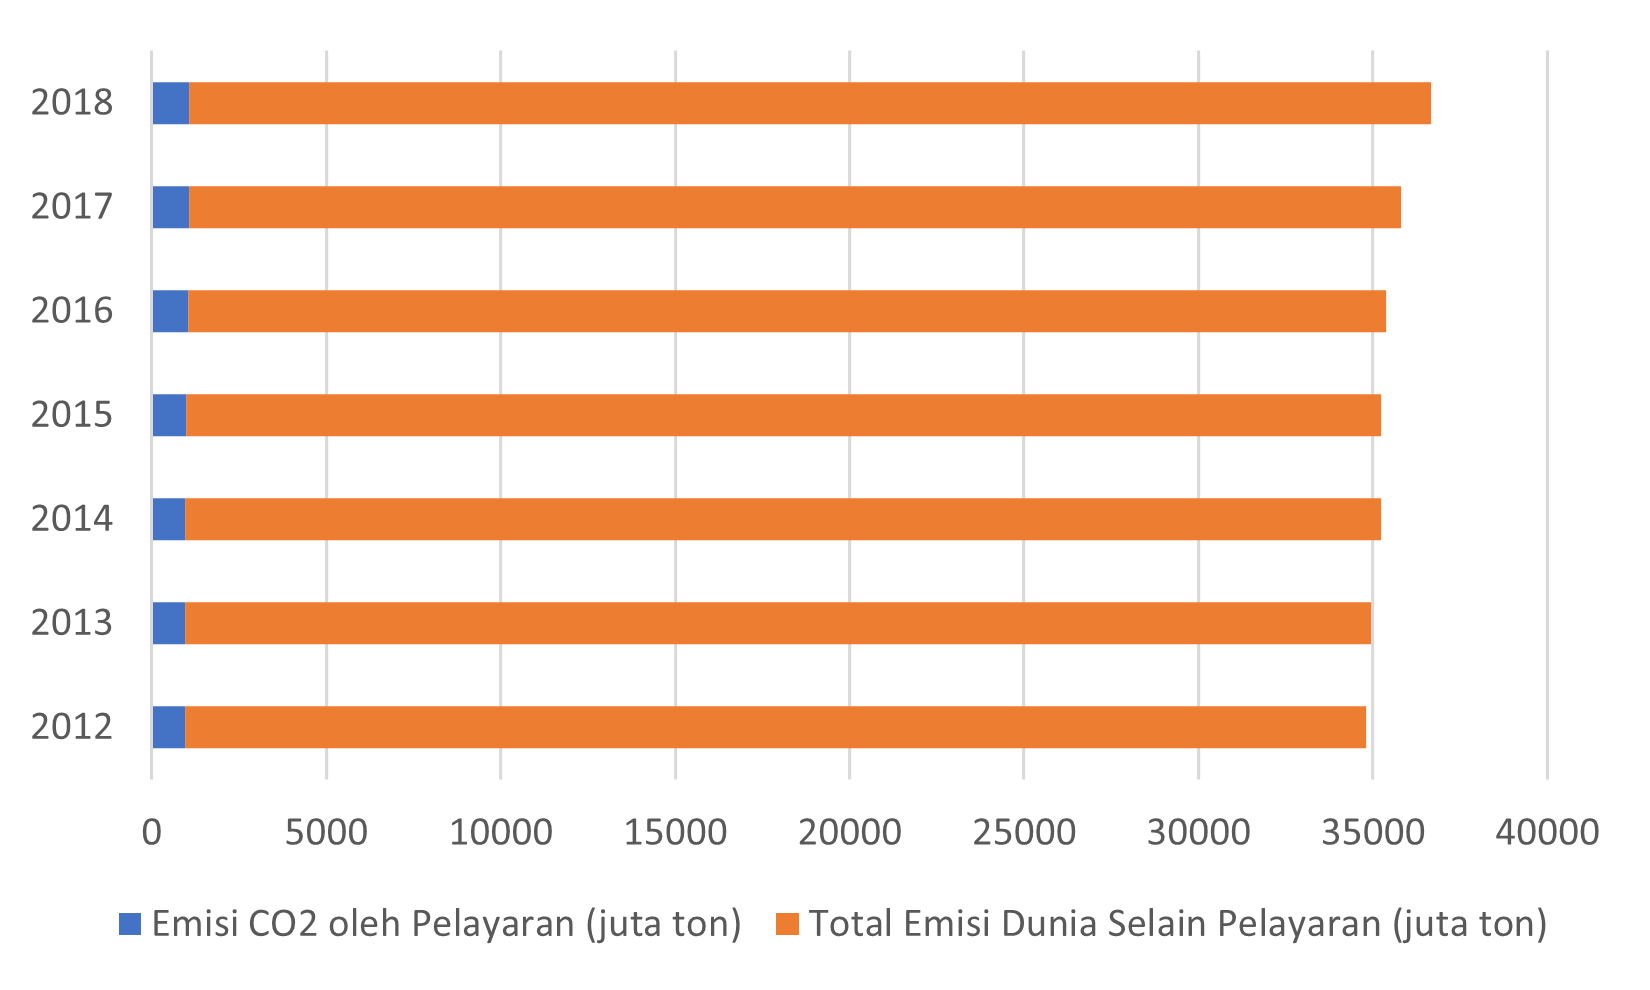
\includegraphics[width=0.95\textwidth,keepaspectratio]{gambar/grafik-emisi-LB.png}
  \caption{Grafik Perbandingan Emisi Karbon Pelayaran dengan Total Emisi Karbon Dunia \citep{unctadREVIEWMARITIMETRANSPORT2021}.}
  \label{fig:grafikemisidunia}
\end{figure}

Salah satu sektor yang diharapkan mampu bertransformasi adalah sektor pelayaran. Transportasi laut memegang peranan penting dalam ekonomi global. Berdasarkan data dari UNCTAD pada tahun 2020 lebih dari 82\% perdagangan dunia dilayani oleh transportasi laut \citep{unctadREVIEWMARITIMETRANSPORT2021}.
Volume barang yang diangkut pada tahun 2021 meningkat sebesar 40.5\% dibandingkan dengan tahun 2010. Jasa angkutan laut tumbuh dengan nilai rata-rata 2\% tiap tahunnya sejak tahun 1970. Sektor pelayaran menyumbang 3\% dari keseluruhan emisi karbon dunia. Angka tersebut diperkirakan akan terus tumbuh berbanding lurus dengan pertumbuhan nilai perdagangan dunia. Hal tersebut dapat dilihat pada Gambar \ref{fig:grafikemisidunia}

Penanganan gas rumah kaca masih menjadi polemik dunia saat ini. Meskipun semua pihak sudah sepakat bahwa GRK harus segera dikurangi namun belum ada kesepakatan yang jelas mengenai cara dan pihak yang bertanggungjawab terhadap fenomena GRK \citep{gritsenkoRegulatingGHGEmissions2017}.
Penanganan GRK hasil emisi pelayaran membutuhkan pendekatan yang tepat dikarenakan dalam kondisi saat ini GRK merupakan produk utama pelayaran selain dari jasa transportasi itu sendiri. Pengurangan GRK pada industri pelayaran akan sangat mempengaruhi operasional dan ekonomi sektor ini. Sebagi contoh pergantian bahan bakar dari \emph{Heavy Fuel Oil} menuju \emph{Liquid Natural Gas} akan berdampak langsung pada kapasitas angkut kapal, pelabuhan yang dapat melayani kapal tersebut dan biaya bahan bakar.

Meskipun masih dibayang-bayangi ketidakpastian mengenai angka standar yang disepakati, beberapa regulasi pengurangan karbon kapal sudah diratifikasi oleh IMO dan bersifat mengikat. Sebagai contoh adalah regulasi \emph{Carbon Intensity Indicator} yang membatasi berapa karbon yang dihasilkan kapal tiap unit transportasinya. Kapal yang tidak mampu memenuhi batas yang sudah ditentukan oleh IMO akan diberikan peringatan untuk memperbaiki atau memilih untuk dicabut izin operasinya oleh IMO \citep{qiBilevelOptimizationModel2021}.
Hal ini menggambarkan urgensitas perusahaan pelayaran domestik untuk segera mempersiapkan akan regulasi yang akan datang ini demi kelancaran dalam operasionalnya.

Singapura memiliki kedudukan yang sangat penting bagi dunia pelayaran Indonesia. Peran utama Singapura sebagai penghubung pelayaran internasional dan juga sebagai gerbang utama rantai pasok Indonesia. Hal ini ditunjukkan dengan posisi Indonesia sebagai sepuluh besar negara dengan jumlah kapal yang singgah di Singapura \citep{rusliProtectingVitalSea2012}.
Singapura sudah merancang strategi pengurangan karbon dari pelayaran yang dituangkan dalam \emph{Maritime Singapore
Decarbonisation Blueprint: Working Towards 2050}. Tidak berhenti sampai disitu, Singapura juga menyiapkan 300 juta USD demi mewujudkan rencana tersebut. Hal yang perlu diperhatikan adalah sangat besar peluang Singapura menjadi pionir utama dalam penerapan regulasi karbon ini. Pelayaran Indonesia menjadi pihak langsung yang akan terdampak dari regulasi atau kebijakan baru yang akan diterapkan oleh Singapura. Langkah tepat harus diambil dan disiapkan oleh perusahaan pelayaran Indonesia demi menghadapi hal tersebut.

Interaksi dan dampak dari diterapkannya suatu kebijakan atau inovasi pengurangan GRK dalam bidang pelayaran perlu diteliti untuk melakukan proyeksi dari inovasi pengurangan karbon yang dapat digunakan dan keputusan untuk melanjutkan operasional sebuah kapal. Salah satu metode yang dapat digunakan untuk memotret hubungan tersebut adalah dinamika sistem. Metode dinamika sistem sebelumnya sudah digunakan untuk meneliti masalah keberlanjutan, dimana tidak ada solusi yang pasti dan linear \citep{hjorthNavigatingSustainableDevelopment2006}. Maka oleh karena itu penelitian mengenai dampak kebijakan pengurangan emisi gas rumah kaca dengan pendekatan dinamika sistem perlu dilakukan.
\end{comment}